% Generated by tools/figures.mjs from analysis/position-adjust-6model-2026-10-09.json - do not edit by hand.
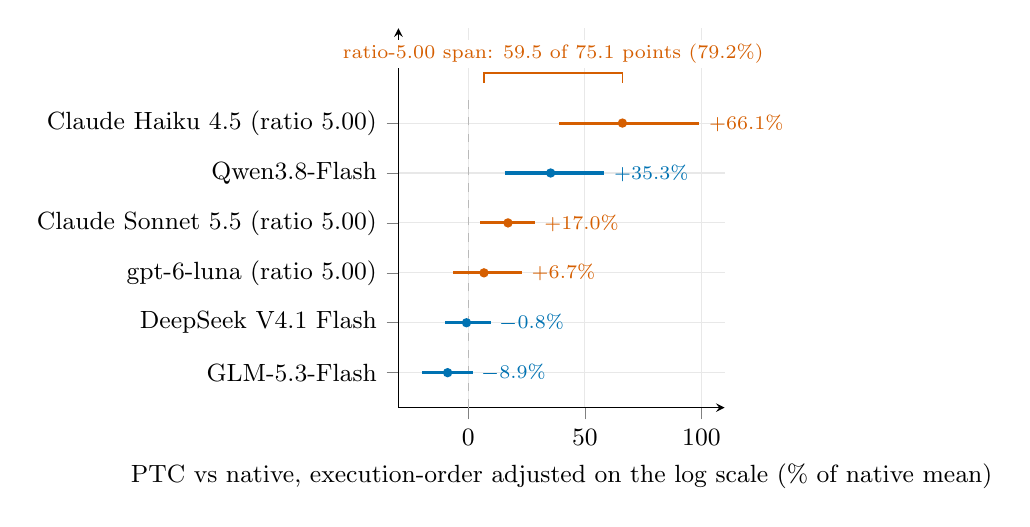
\begin{tikzpicture}
\definecolor{f1main}{HTML}{0072B2}
\definecolor{f1r5}{HTML}{D55E00}
\begin{axis}[
  width=\linewidth-6.4cm, height=6.4cm, compat=1.18,
  xlabel={PTC vs native, execution-order adjusted on the log scale (\% of native mean)},
  xmin=-30, xmax=110,
  ytick={0,1,2,3,4,5},
  yticklabels={GLM-5.3-Flash,DeepSeek V4.1 Flash,gpt-6-luna (ratio 5.00),Claude Sonnet 5.5 (ratio 5.00),Qwen3.8-Flash,Claude Haiku 4.5 (ratio 5.00)},
  yticklabel style={font=\small}, xticklabel style={font=\small}, xlabel style={font=\small}, ylabel style={font=\small},
  ymin=-0.7, ymax=6.9,
  axis y line=left, axis x line=bottom, tick align=outside,
  grid=major, grid style={gray!18},
  clip=false,
]
\draw[gray!55, dashed] (axis cs:0,-0.7) -- (axis cs:0,5.6);
\draw[f1r5, line width=0.6pt] (axis cs:6.7,5.8) -- (axis cs:6.7,6.0) -- (axis cs:66.1,6.0) -- (axis cs:66.1,5.8);
\node[font=\scriptsize, anchor=south, text=f1r5, fill=white, inner sep=1.5pt] at (axis cs:36.4,6.1) {ratio-5.00 span: 59.5 of 75.1 points (79.2\%)};
\draw[f1main, line width=1.1pt] (axis cs:-20.0,0) -- (axis cs:1.8,0);
\node[circle, fill=f1main, inner sep=1.2pt] at (axis cs:-8.9,0) {};
\node[font=\scriptsize, anchor=west, text=f1main] at (axis cs:1.8,0) {\textminus{}8.9\%};
\draw[f1main, line width=1.1pt] (axis cs:-10.0,1) -- (axis cs:9.6,1);
\node[circle, fill=f1main, inner sep=1.2pt] at (axis cs:-0.8,1) {};
\node[font=\scriptsize, anchor=west, text=f1main] at (axis cs:9.6,1) {\textminus{}0.8\%};
\draw[f1r5, line width=1.1pt] (axis cs:-6.5,2) -- (axis cs:23.0,2);
\node[circle, fill=f1r5, inner sep=1.2pt] at (axis cs:6.7,2) {};
\node[font=\scriptsize, anchor=west, text=f1r5] at (axis cs:23.0,2) {+6.7\%};
\draw[f1r5, line width=1.1pt] (axis cs:5.0,3) -- (axis cs:28.4,3);
\node[circle, fill=f1r5, inner sep=1.2pt] at (axis cs:17.0,3) {};
\node[font=\scriptsize, anchor=west, text=f1r5] at (axis cs:28.4,3) {+17.0\%};
\draw[f1main, line width=1.1pt] (axis cs:15.6,4) -- (axis cs:58.3,4);
\node[circle, fill=f1main, inner sep=1.2pt] at (axis cs:35.3,4) {};
\node[font=\scriptsize, anchor=west, text=f1main] at (axis cs:58.3,4) {+35.3\%};
\draw[f1r5, line width=1.1pt] (axis cs:39.1,5) -- (axis cs:99.1,5);
\node[circle, fill=f1r5, inner sep=1.2pt] at (axis cs:66.1,5) {};
\node[font=\scriptsize, anchor=west, text=f1r5] at (axis cs:99.1,5) {+66.1\%};
\end{axis}
\end{tikzpicture}
